\documentclass[smallextended]{svjour3}       % onecolumn (second format)
%\documentclass[twocolumn]{svjour3}          % twocolumn
%
\smartqed  % flush right qed marks, e.g. at end of proof
%
\usepackage{graphicx}
\usepackage{epstopdf}
\usepackage[latin9]{inputenc}
\usepackage{float}
\usepackage{amsmath}
\usepackage{amssymb}
\usepackage{esint}
\usepackage{array}
\usepackage[colorlinks=true, urlcolor=citecolor, linkcolor=citecolor, citecolor=citecolor]{hyperref}
%\usepackage{subcaption}
\usepackage{subfig}
\usepackage[]{natbib}
\makeatletter

%%%%%%%%%%%%%%%%%%%%%%%%%%%%%% LyX specific LaTeX commands.
%% Because html converters don't know tabularnewline
\providecommand{\tabularnewline}{\\}

%%%%%%%%%%%%%%%%%%%%%%%%%%%%%% User specified LaTeX commands.
\newcommand{\X}{{\mathsf{X}}}

%
% \usepackage{mathptmx}      % use Times fonts if available on your TeX system
%
% insert here the call for the packages your document requires
%\usepackage{latexsym}
% etc.
%
% please place your own definitions here and don't use \def but
% \newcommand{}{}
%
% Insert the name of "your journal" with
% \journalname{myjournal}
%
\begin{document}

\title{Bayesian analysis of survival data under generalized extreme value distribution with application in cure rate model}
%\subtitle{Do you have a subtitle?\\ If so, write it here}

\titlerunning{Bayesian analysis of survival data with GEV}        % if too long for running head

\author{
}

\authorrunning{} 
% if too long for running head

\institute{
}

\date{Received: date / Accepted: date}
% The correct dates will be entered by the editor


\maketitle

\begin{abstract}
This paper introduces both maxima and minima generalized extreme value (GEV) distribution
to analyze right-censored survival data with a cure fraction. Our proposed GEV model leads to extremely flexible hazard functions. Our proposed Bayesian model achieves proper posterior distribution under some weak conditions when improper priors are used. We further provide theoretical and numerical results showing that our GEV models offer a richer class of models than the widely used Weibull models. Finally, a glioblastoma multiforme cancer data is analyzed to illustrate the proposed GEV model.
\keywords{Cure fraction \and Generalized extreme value distribution \and Gibb's sampler \and MCMC \and Metropolis Hastings \and Survival analysis \and Real data analysis \and Seer \and Glioblastoma Multiforme \and Melanoma of the skin}
% \PACS{PACS code1 \and PACS code2 \and more}
% \subclass{MSC code1 \and MSC code2 \and more}
\end{abstract}

\section{Introduction}
\label{sec:intro}
%\noindent
Ever since 1936, when Richard Von Mises had studied Extreme Value Theory (EVT) for the very first time, it has become a popular tool to model risk as risky events by definition happen with low probability. Today Generalized Extreme Value (GEV) distribution finds its use across several disciplines like reliability, hydrology, meteorology and finance. However its usefulness in survival modeling domain remains unexplored. 
In \citet{roy:dey:2014}, the authors show that GEV gives rise to extremely flexible hazard functions with slight variations of the scale and the shape parameters. This flexible hazard functions will be useful in several practical situations. For example, when studying the disease span of a relapsed leukemia cancer patient, it is quite possible that a three-phase behavior of the failure rate will be observed. The initial risk of survival before the cancer reacts to medications, achieves remission and then after a span relapses. Similar remission and relapse patterns are also observed in other cancer types like lymphoma. A model with a bathtub or ``U''
shaped failure rate would be appropriate to describe such a  population's survival capacity. Extending the results of \citet{roy:dey:2014} in this article, we build flexible survival models using both the maxima and minima GEV distribution for log T, where T denotes the failure time/ survival time of an individual. We are able to show that by changing the shape parameter of the GEV distribution, a variety of shape for the hazard function including upside-down and bathtub shapes are obtained. 

%\noindent
During the last two decades, several cancer related studies have demonstrated
that a significant fraction of the diseased population has been cured.
This can be attributed to the development of the advanced medical techniques as well
as timely diagnosis of the cancer. It is due to this fact, that survival
models incorporating a cure fraction have gained significant attention and importance
in the literature. We use the log GEV survival models mentioned above to construct flexible cure rate model.


The cure rate model is popularly used for modeling time-to-event survival
data. Perhaps the most popular type of cure rate model is the mixture
model introduced by \citet{berk:gage:1952} around 60 years ago. 
This binary mixture model has played an important role in the literature and has been discussed by multiple authors
including \citet{farewell:1982}, \citet{kuk:chen:1992}, \citet{maller:zhou:1996},
 \citet{peng:dear:2000} and \citet{sy:taylor:2000} among others.


In \citet{chen:ibra:sinh:1999}, it is shown that the cure rate
model discussed above has several drawbacks and the authors proposed a different kind of cure
rate model. This proposed model has a proportional hazards structure
through the cure rate parameter, and thus has an appealing
interpretation. Unlike the standard cure rate
model, the model in \citet{chen:ibra:sinh:1999} yields proper posterior distributions under
a wide class of non-informative improper priors for the regression
coefficients, including an improper uniform prior. Also
by introducing latent variables, posterior samples for parameters can
be efficiently obtained for this model.


In \citet{chen:ibra:sinh:1999}, the proposed model uses Gamma and
Weibull distributions, which are quite popular with monotone hazard
rates. However, it is well known that in practical situations for survival
analysis, the hazard function is often not monotone and is either
upside-down shaped or bathtub shaped or a combination of both shapes.


In this paper, we introduce cure rate models using GEV distributions. 
We use Bayesian methodology to do the inference for
parameters. An important issue in Bayesian analysis is the specification
of a prior distribution. This is especially true in survival analysis
when one wants to assess the importance of certain prognostic factors
such as age, gender, etc. It may be difficult to specify informative
priors for all possible candidate models, especially if little prior
information is available. When such prior elicitation is difficult
or when little prior information is available, one may consider analyses
with conventionally chosen non-informative priors, such as the improper uniform prior.
We provide sufficient conditions
under which the joint posterior distribution of the parameters of interest
is proper when improper uniform prior is used for regression parameters
for covariates incorporated through the cure rate parameter. This
prior is analytically and computationally attractive and facilitates
a direct comparison with maximum likelihood.


The article is organized as follows. In Section 2 we provide an
introduction to the standard log generalized extreme value distribution
for maxima and minima and demonstrate their flexibility through plots of hazard functions. In Section 3 we derive the likelihood function for cure rate models 
with covariates and consider a useful class of non informative prior distributions.
We also derive several results regarding
proprieties of the resulting posterior distributions. In Section 4
we consider some numerical simulation examples. In this section
we compare both GEV maxima and minima models with the Weibull distribution model to show
the superiority of our proposed models. We carry out model selection using Deviance
Information Criterion (DIC) and Log Pseudo Marginal Likelihood (LPML) measures and also
compute the model diagnostics for GEV minima (mGEV) model under perturbation.
In Section 5 we present a real glioblastoma multiforme data set from SEER (\citet{seer:database:2013}) to illustrate our proposed methodology. We conclude with a brief discussion in Section 6. Supplementary materials contains proofs of some of the theorems and another real data example using a melanoma cancer data set.
\section{Generalized extreme value distribution}

\subsection{Introduction to the Generalized extreme value distribution}
\label{sec:gev}
%\noindent
Suppose $Y_{1},Y_{2},...$ is a sequence of independent and identically
distributed random variables each having the distribution function
$F(y)$. Let $M_{n}$ = $\max\{Y_{1},Y_{2},...,Y_{n}\}$ and $m_{n}=\min\{Y_{1},Y_{2},...,Y_{n}\}$.
If the distribution of $Y_{i}$ is specified then the exact distributions
of $M_{n}$ and $m_{n}$ are known. Besides, extreme value theory
also considers the existence of the limiting distributions of $M_{n}$
and $m_{n}$. If there exists a non-degenerate distribution function
$G_{\xi}(x)$, and a pair of sequences ${a_{n}},{b_{n}},$with $a_{n}>0$,
such that
\begin{equation}
\lim_{n\rightarrow\infty}P\{a_{n}^{-1}(M_{n}-b_{n})\leq x\}=G_{\xi}(x)
\end{equation}
%\noindent
on all points in the continuity set of $G_{\xi}(x)$, we say that
$G_{\xi}(x)$ is a generalized extreme value distribution for maxima.
The possible forms of $G_{\xi}(x)$ are completely specified as follows:
\[
G_{\xi}(x)=\begin{cases}
\exp[-(1+\xi\frac{x-\mu}{\sigma})_{+}^{-\frac{1}{\xi}}] & \ \mbox{if}\ \xi>0\ \mbox{or}\ \xi<0\\
\exp[-\exp(-\frac{x-\mu}{\sigma})] & \ \mbox{if}\ \xi=0,
\end{cases}
\]
%\noindent
where $\mu\in R$, $\sigma\in R^{+}$, and $\xi\in R$ are the location,
scale, and shape parameters respectively, and $x^{+}=\mbox{max}(x,0)$.
%\noindent
Similarly, we could get the limiting distribution of $m_{n}$, called
the generalized extreme value distribution for minima.
%\noindent
Cumulative distribution function of the GEV distribution for minima
is given by:
\[
G_{\xi}(x)=\begin{cases}
1-\exp[-(1+\xi\frac{x-\mu}{\sigma})_{+}^{\frac{1}{\xi}}] & \ \mbox{if}\ \xi>0\ \mbox{or}\ \xi<0\\
1-\exp[-\exp(\frac{x-\mu}{\sigma})] & \ \mbox{if}\ \xi=0,
\end{cases}
\]
%\noindent
where $\mu\in R$, $\sigma\in R^{+}$, and $\xi\in R$ are the location,
scale, and shape parameters, respectively.
In their book \citet{castillo:hadi:2004}, the authors provide many real life applications of extreme value distribution in disciplines such as structural engineering, hydraulics, meteorology, materials science, highway traffic analysis, environmetrics and climatology. 


\subsection{Shape of Hazard function for the logGEV distribution}
%\noindent
Going forward, we will use the notations MGEV and mGEV for representing the GEV maxima model and the GEV minima
model respectively.


If we assume a MGEV distribution for $\log$ T, i.e., $\log T\sim\mbox{MGEV}(\mu,\sigma,\xi)$
, then we write $\mbox{T}\sim\log MGEV(\mu,\sigma,\xi)$. The corresponding cdf and pdf for T are respectively

\[
F_M(t|\mu,\sigma,\xi)=\Psi_{MGEV}\bigg(\frac{\log(t)-\mu}{\sigma}\bigg),
\]

\[
f_M(t|\mu,\sigma,\xi)=\frac{1}{\sigma t}\psi_{MGEV}\bigg(\frac{\log(t)-\mu}{\sigma}\bigg),
\]
%\noindent
where $\Psi_{MGEV}$ and $\psi_{MGEV}$ are the cdf and pdf respectively for the standardized MGEV distribution.

In other words,
\[
f_M(t|\mu,\sigma,\xi)=\begin{cases}
\frac{\exp[-(1+\xi\frac{\log t-\mu}{\sigma})^{-\frac{1}{\xi}}]}{\sigma t(1+\xi\frac{\log t-\mu}{\sigma})^{\frac{1}{\xi}+1}} & t>\exp(\mu-\frac{\sigma}{\xi})\ \mbox{if}\ \xi>0 \:or\\
\                                                                                                                           & t<\exp(\mu-\frac{\sigma}{\xi})\ \mbox{if}\ \xi<0\\
\frac{1}{\sigma t}\exp(-\frac{\log t-\mu}{\sigma})\exp[-\exp(-\frac{\log t-\mu}{\sigma})]  & 0<t<\infty\ \mbox{if}\ \xi=0
\end{cases}
\]
%\noindent
and the survival function, which is $1-F_M(t|\mu,\sigma,\xi)$, is given by,
\[
S_M(t|\mu,\sigma,\xi)=\begin{cases}
1-\exp[-(1+\xi\frac{\log t-\mu}{\sigma})_{+}^{-\frac{1}{\xi}}]\  & \mbox{if}\ \xi\neq0\\
1-\exp(-\exp(-\frac{\log t-\mu}{\sigma})) & \mbox{if}\ \xi=0
\end{cases}
\]
%\noindent
In the special case when $\mu=0$ and $\sigma=1$ {as mentioned in  \citet{roy:dey:2014}, the density of T is
\[
f_M(t|\xi)=\begin{cases}
\frac{\exp[-(1+\xi\log t)^{-\frac{1}{\xi}}]}{t(1+\xi\log t)_{+}^{\frac{1}{\xi}+1}} & \mbox{if} \xi\neq 0\\
\frac{1}{t^{2}}\exp(-\frac{1}{t}) & 0<t<\infty\ \mbox{if}\ \xi=0,
\end{cases}
\]
%\noindent
and the corresponding survival function is
\[
S_M(t|\xi)=\begin{cases}
1-\exp[-(1+\xi\log t)_+^{-\frac{1}{\xi}}]\  & \mbox{if}\ \xi\neq0\\
1-\exp(-\frac{1}{t}) & \mbox{if}\ \xi=0.
\end{cases}
\]

%\noindent
Hence, the corresponding hazard function $\lambda_M(t|\xi)=f(t|\xi)/S(t|\xi)$ is given by

\[
\lambda_M(t|\xi)=\begin{cases}
\frac{1}{t(1+\xi\log t)_+^{\frac{1}{\xi}+1}[\exp(1+\xi\log t)_+^{-\frac{1}{\xi}}-1]} & \ \mbox{if}\ \xi\neq0\\
\frac{1}{t^{2}[\exp(\frac{1}{t})-1]} & \ \mbox{if}\ \xi=0.
\end{cases}
\]


%\noindent
Figure 1(a) and 1(b) show the plots of the hazard function of $\mbox{MGEV}(\mu=0,\sigma,\xi)$ where $\sigma = 1$ for 1(a) and $\sigma = 1.5$ in case of 1(b) for five different values of $\xi$. \citet{roy:dey:2014} used plot 1(a) to show that the MGEV model is extremely flexible in modeling survival data. 


On the other hand, if we assume a mGEV distribution for log T, i.e.,  $\mbox{log T}\sim\mbox{mGEV}(\mu,\sigma,\xi)$, the corresponding cdf and pdf for T are

\[
F_m(t|\mu,\sigma,\xi)=\Psi_{mGEV}\bigg(\frac{\log(t)-\mu}{\sigma}\bigg),
\]


\[
f_m(t|\mu,\sigma,\xi)=\frac{1}{\sigma t}\psi_{mGEV}\bigg(\frac{\log(t)-\mu}{\sigma}\bigg),
\]

%\noindent
where $\Psi_{mGEV}$ and $\psi_{mGEV}$ are the cdf and pdf respectively for the standardized mGEV distribution.

When $\mu=0$ and $\sigma=1$, the density of T could be written as:

\[
f_m(t|\xi)=\begin{cases}
\frac{1}{t}(1+\xi\log t)_{+}^{\frac{1}{\xi}-1}\exp[-(1+\xi\log t)_{+}^{\frac{1}{\xi}}] & \mbox{if} \xi \neq 0\\
\exp(-t) & 0<t<\infty\ \mbox{if}\ \xi=0.
\end{cases}
\]

The corresponding survival and the hazard functions respectively are given as follows,
\[
S_m(t|\xi)=\begin{cases}
\exp[-(1+\xi\log t)_{+}^{\frac{1}{\xi}}]\  & \mbox{if}\ \xi\neq0\\
\exp(-t) & \mbox{if}\ \xi=0,
\end{cases}
\]


\[
\lambda_m(t|\xi)=\begin{cases}
\frac{1}{t}(1+\xi\log t)_{+}^{\frac{1}{\xi}-1}\  & \mbox{if}\ \xi\neq0\\
1 & \mbox{if}\ \xi=0.
\end{cases}
\]


Figure 1(c) shows the plot of the above hazard function of $\mbox{mGEV}(\mu=0,\sigma=1,\xi)$
for five different values of $\xi = -0.03,0,0.03.,0.05,-0.05$ Note that when $\xi=0$, this is the hazard from of $\mbox{Weibull}(1,1)$
(See lemma 1 in Section 4.2). Although the value of $\xi$ changes only slightly, the hazard functions change
significantly, especially when the time-to-failure is very small. Figure 1(d) shows the plot of the hazard function of $\mbox{mGEV}(\mu=0,\sigma=1.5,\xi)$
with the same five $\xi$  values as figure 1(c). Note that the
change of the scale parameter $\sigma$ results in totally different shapes of the plot for hazard functions from that in Figure 1(c). Thus
the $\mbox{mGEV(\ensuremath{\mu},\ensuremath{\sigma},\ensuremath{\xi}) }$ distribution leads to
extremely flexible hazard functions.

\section{Modeling log survival data with a cure fraction with GEV distributions}
\label{sec:sur}
Cure rate models have been used for modeling time-to-event data for
various types of cancers. For some specific cancer types, a significant proportion
of patients are experiencing complete remission or are being ``cured'' after treatment. As mentioned in the introductory section, in the popular 
standard cure rate model (\citet{berk:gage:1952}) the survival function for
the entire population, denoted by $S_{1}(t)$, is given by $S_{1}(t)=\pi+(1-\pi)S^{*}(t),$
where a fraction $\pi$ of the population are considered ``cured''
and the remaining $1-\pi$ are ``non-cured'', and $S^{*}(t)$ denotes
the survival function for the non-cured group in the population.
This model, though attractive, still has several drawbacks. For
example, when including covariates through $\pi$, we might get improper
posterior distributions for many types of non-informative improper
priors. This is a serious drawback, since a proper posterior is required
if we want to perform Bayesian inference. To overcome the drawbacks
of the standard cure rate model, a different type of cure rate model is
introduced in \citet{chen:ibra:sinh:1999} and the specified
distribution is the Weibull distribution. In Lemma 1, it is proved that
the logarithm of the Weibull distribution is a special case of the generalized
extreme value distribution. In this paper, we apply the logarithm of the generalized
extreme value distribution to the model given in \citet{chen:ibra:sinh:1999} to incorporate a larger class of models.


Suppose that we have $n$ subjects, and let $N_{i}$ denote the number
of clonogenic cells for the $i$th subject. Further, assume that
the $N_{i}$'s are i.i.d. Poisson random variables with mean $\theta_{i}$,
$i=1,\ldots,n$. We emphasize here that the $N_{i}$'s are not observed
and can be viewed as latent variables. The incubation times
for the $N_{i}$ clonogenic cells for the $i$th subject, which
are unobserved, are assumed to be i.i.d. with common cdf $F(\cdot)$,$\ i=1,\ldots,n$. Let
$t_{i}$ denote the failure time for subject $i$, where $t_{i}$
is right-censored. Let $c_{i}$ denote the censoring time, so that
we observe $y_{i}=\mbox{min}(t_{i},c_{i})$, where the censoring
indicator $\delta_{i}=I(t_{i}<c_{i})$ equals $1$ if $t_{i}$ is
a failure time and $0$ if it is right-censored. We represent the observed
data by the vector $(n,\mathbf{y},\delta)$, where $\mathbf{y}=(y_{1},\cdots,y_{n})$
and $\mathbf{\delta}=(\delta_{1},\cdots,\delta_{n})$. Also, let $\mathbf{N}=(N_{1},\cdots,N_{n}),$
$\boldsymbol{\theta}=(\theta_{1},\cdots,\theta_{n})$. The complete data
are then given by $\mathbf{D}=(n,\mathbf{y},\mathbf{\delta},\mathbf{N})$,
where $\mathbf{N}$ is the unobserved vector of latent variables. We
assume the density for $y_{i}$ is $f(y_{i}|\xi)$ and the corresponding
survival function is $S(y_{i}|\xi).$ Here, $\xi$ is the shape parameter
in the standard MGEV or mGEV distribution which we will
use later.
The complete data likelihood function of the parameters $(\boldsymbol{\theta},\xi)$
can be written as
\begin{equation}
L(\boldsymbol{\theta},\xi|D) = \prod_{i=1}^{n}S(y_{i}|\xi)^{N_{i}-\delta_{i}}(N_{i}f(y_{i}|\xi))^{\delta_{i}}\times \exp\Big\{\sum_{i=1}^{n}(N_{i}\log(\theta_{i})-\log(N_{i}!)-\theta_{i})\Big\}.\label{eq:f}
\end{equation}
%%\noindent
Now we incorporate the covariates through $\mathbf{\theta}$. For each
subject, $i=1,\cdots,n$, let $\mathbf{x}_{i}^{\prime}=(x_{i1},\cdots,x_{ik})$
denote the $k\times1$ vector of covariates for the $i$th subject,
and let $\boldsymbol{{\beta}}=(\beta_{1},\cdots,\beta_{k})$ denote
the corresponding vector of regression coefficients. We relate $\boldsymbol{\theta}$
to the covariates by $\theta_{i}=\exp(\mathbf{x}_{i}^{\prime}\mathbf{\beta}),\ i=1,\cdots,n.$ 
so that the chance of cure for the $i'$th subject is given by $P(N_i = 0) = \exp(-\theta_i) = \exp(-\exp(\mathbf{x}_{i}^{\prime}\mathbf{\beta}))$.
%%\noindent
Thus we could write the complete-data likelihood of $(\beta,\xi)$
as
\begin{eqnarray}
L(\boldsymbol{\beta},\xi|\mathbf{D}) & = & \prod_{i=1}^{n}S(y_{i}|\xi)^{N_{i}-\delta_{i}}(N_{i}f(y_{i}|\xi))^{\delta_{i}}\times\exp\Big\{N_{i}\mathbf{x}_{i}^{\prime}\boldsymbol{\beta}-\log(N_{i}!)-\exp(\mathbf{x}_{i}^{\prime}\boldsymbol{\beta})\Big\}.\label{eq:h}
\end{eqnarray}
%\noindent
Assume that the prior distribution for $(\beta,\xi)$ is $\pi(\beta,\xi)$,
then the posterior distribution $\pi(\beta,\xi|\mathbf{D}_{obs})$
satisfy this:
\begin{eqnarray}
\pi(\mathbf{\beta},\xi|\mathbf{D}_{obs}) & \varpropto & \sum_{\mathbb{N}}L(\mathbf{\beta},\xi|\mathbb{\mathbf{D}})\pi(\mathbf{\beta},\xi).\label{eq:a}
\end{eqnarray}

\subsection{MGEV Distribution for Right-Censored Data}\label{sec1}
\noindent
Let $t_{i}$ be the failure time for the $i'$th subject. Let $c_{i}$ be the censoring time. Then
$y_{i}$ = min($t_{i}$,$c_{i});i=1,..,n$. Assume that $\log y_{i}\sim\mbox{MGEV}(\mu=0,\sigma=1,\xi)$.
We use an improper uniform prior on $\beta$, that is, $\pi(\mathbf{\beta})\varpropto1$,
and the prior on $\xi$ is $\pi(\xi)= 1/(b-a) I_{[a,b]}(\xi)$,where $a<0<b$,
are fixed numbers. We also assume that $\pi(\mathbf{\beta},\xi)=\pi(\mathbf{\beta})\cdot\pi(\xi)$.

\begin{theorem} \label{thm:1-1}
Let $\mathbb{\mathbf{X}}^{*}$ be
an $n\times k$ matrix with rows $\delta_{i}\mathbf{x}_{i}^{\prime}$.
If the following two conditions hold:

\begin{enumerate}
\item $\mathbb{\mathbf{X}}^{*}$ is of full rank,
\item For every $i$ with $\delta_{i}=1,$
\begin{equation}
\exp(- 1/ b)< y_{i} < \exp(- 1/a)\ ;\mbox{or}\; y_{i}\geq\max(\exp(-1/a),e),\label{eq:s}
\end{equation}
\end{enumerate}
then the posterior distribution given in (\ref{eq:a}) is proper.
\end{theorem}
\noindent
The proof of the Theorem \ref{thm:1-1} is given in the supplementary materials.

\begin{remark}
  \label{rem:cond}
  If $\log y \sim\mbox{MGEV}(0,1,\xi)$, then $1+ \xi \log y >0$, that
  is, $y > \exp(- 1/\xi)$ if $\xi >0$ and $y < \exp(- 1/\xi)$ if $\xi
  <0$. Hence, the condition $\exp(- 1/ b)< y_{i} < \exp(- 1/a)$ in
  \eqref{eq:s} is natural as the support of the prior distribution of
  $\xi$ includes the points $a$ and $b$.
\end{remark}

\begin{remark}

  If $a=-b$ \& $0<b\leq1$, (\ref{eq:s}) changes to $y_{i}>\exp(- 1/
  b)$.  This is a relatively weaker condition.  If $a=-b$ \& $b>1$,
  (\ref{eq:s}) changes to
  $\exp(-1/b)<y_{i}<\exp(-1/b)\ \;\mbox{or}\;
  y_{i}\geq e$ .
\end{remark}
In the special case when $b=-a=1$, that is, when $\pi(\xi)= (1/2)I_{[-1,1]}(\xi)$, we have the following
corollary.
\begin{corollary}
\label{thm:1}
\noindent
Let $\mathbb{\mathbf{X}}^{*}$ be
an $n\times k$ matrix with rows $\delta_{i}\mathbf{x}_{i}^{\prime}$.
If the following two conditions hold:
\begin{enumerate}
\item $\mathbb{\mathbf{X}}^{*}$ is of full column rank,
\item For every $i$ with $\delta_{i}=1$, $y_{i}> 1/e$,
\end{enumerate}
\noindent
then the posterior distribution given in (\ref{eq:a}) is proper.
\end{corollary}

Now we use the following prior on $\xi$: $\pi(\xi)=c\exp(- |\xi| /2),\
-a< \xi <a, a>0$, along with the previously used uniform prior on
$\beta$. Simple calculations show that $c=4(1-\exp(- a/2))$. The
following theorem provides sufficient conditions for posterior propriety
in this case. Our goal is to show that the posterior attains propriety under
different reasonable priors.
\begin{theorem} \label{thm:1-1-1}
Let $\mathbb{\mathbf{X}}^{*}$ be
an $n\times k$ matrix with rows $\delta_{i}\mathbf{x}_{i}^{\prime}$.
If these two conditions hold:
\begin{enumerate}
\item $\mathbb{\mathbf{X}}^{*}$ is of full column rank,
\item For every $i$ with $\delta_{i}=1$,
\end{enumerate}
\begin{equation}
\exp(-1/a)< y_{i} <\exp(1/a)\ \; \mbox{or} \; y_{i}\geq\max(\exp(1/a), e),\label{eq:s-1}
\end{equation}
then the posterior distribution given in (\ref{eq:a}) is proper.
\end{theorem}
\noindent
The proof of the Theorem \ref{thm:1-1-1} is similar to that of Theorem 1 and hence omitted.

\subsection{mGEV Distribution for Right-Censored Data}
 As in Section \ref{sec1}, we can establish sufficient conditions under which the posterior density \eqref{eq:a} is proper
 when a mGEV distribution for $\log y_{i}$ is used. Consider the uniform
prior for $\xi$ on $(a, b)$, that is, $\pi(\xi)= 1/(b-a) I_{[a,b]}(\xi),\ a<0<b$, and
 $\pi(\mathbf{\beta})\varpropto1$.

\begin{theorem} \label{thm:1-2}
\noindent
Let $\mathbb{\mathbf{X}}^{*}$ be
an $n\times k$ matrix with rows $\delta_{i}\mathbf{x}_{i}^{\prime}$.
If the following two conditions hold:
\begin{enumerate}
\item $\mathbb{\mathbf{X}}^{*}$ is of full column rank,
\item For every $i$ with $\delta_{i}=1$, $\exp(-1/b) < y_{i} < \exp(-1/a)$,
\end{enumerate}
then the posterior distribution given in (\ref{eq:a}) is proper.
\end{theorem}
\noindent
The proof of the Theorem \ref{thm:1-2} is given in supplementary materials. Following the proof of Theorem \ref{thm:1-2}, similar results can be established for other priors on $\xi$
considered in Section \ref{sec1}.

\section{Simulation Studies}
%\noindent
In this section we conduct simulation studies to evaluate model fitting performance along with model comparison, selection and model diagnostics against competing models.
\subsection{Simulation of MGEV model}
%\noindent
Here we simulate a right-censored data set as described in Section
3. The simulation process is given below:

1. Let the sample size be $n=1000$. One covariate (age) and an intercept term are
included in the analysis. Assume $\beta=(1,0.2)^{\prime}$. In the analysis below, we first generate age as a random number between 1 to 100 with replacement and then 
standardized the simulated age to stabilize the posterior computations. So we have the $n\times2$ covariate matrix $X$ with the first column as $1^{'}s$, the second column as the standardized age. Denote the $i$'th row of X by $\mbox{x}_{i}^{'}$, so $\theta_{i}=\exp(\mbox{x}_{i}^{\prime}\boldsymbol\beta),\ i=1,...,n.$. We check that $X$ has full rank. 

2. For every $i$, $i=1,...,n$, we draw a sample from $\mbox{Poisson}(\theta_{i})$,
denoted by $N_{i}$. Then obtain a sample of size $N_{i}$ from $\log MGEV(\mu=0,\sigma=1,\xi=0.3)$, denote them as $Z_{i1},\ldots,Z_{iN_{i}}$.
Set $t_{i}=\min(Z_{i1},\ldots,Z_{iN_{i}}).$ Notice here, if $N_{i}=0$,
then set $t_{i}=\infty.$

3. We take $y_{i}=\mbox{min}(t_{i},c_{i})$ and the indicator $\delta_{i}=I(t_{i}<c_{i})$
equals 1 if $y_{i}$ is a failure time and 0 if it is right-censored. For every $i$, $i=1,...,n$, let $c_{i}$ denote the censoring time. Here, we choose some constant $c_{i}$ so as to let the censoring percentage be close to $23.8\%$. The censoring percentage can be moderated by varying $c_i$. We checked our results using different censoring percentages; from low $5\%$ to high $40\%$, the results were quite similar in terms of accuracy of the estimates and in model comparison. 

4. Next we estimate the parameters using $\mbox{log}T\sim\mbox{MGEV}(\mu=0,\sigma=1,\xi)$
(denoted as the fitting model).

The estimated Kaplan-Meier curve is shown in Figure 2(a), plots the survival function estimate at all simulated survival times using the proposed MGEV model without incorporating any covariate information. We see that the two plots are nearly identical.

We now include covariates in the model and perform a Bayesian analysis. We use a diffused prior on $\beta$ $(\pi(\mathbf{\beta})\varpropto1)$,
and the proper prior on $\xi$ is $\pi(\xi)=\frac{1}{2}I_{[-1,1]}(\xi)$, and assume that $\pi(\mathbf{\beta},\xi)=\pi(\mathbf{\beta})\cdot\pi(\xi)$.
In this example, 10,000 MCMC iterations are used in dealing with the posterior estimation of parameters after a burn-in of 3,000 iterations. Convergence is checked by observing trace plots, autocorrelations and ergodic mean plots (\citet{junk:patz:2013}). The posterior estimates are shown in Table 1. Figure 2(b) shows two box plots of the MLE's of the cure rates and the
posterior estimates of the cure rates. These two estimates of the cure rates are very similar. 

\subsection{Model comparison between mGEV and the Weibull distribution}
%\noindent
We begin with presenting three lemmas which show that the popular Weibull, Rayleigh and the Exponential distributions are special cases of mGEV distribution.
\begin{lemma}
If $T\sim\mbox{Weibull}(\alpha,\lambda)$, then $\log T\sim\mbox{mGEV}(\mu=\log(\lambda),\sigma=\frac{1}{\alpha},\xi=0).$
\end{lemma}\label{lem1}
\begin{lemma}
If $T\sim\mbox{Rayleigh}(\lambda)$, then $\log T\sim\mbox{mGEV}(\mu=\log(\sqrt{2}\lambda),\sigma=\frac{1}{2}, \xi=0).$
\end{lemma}
\begin{lemma}
If $T\sim\mbox{Exponential}(\lambda)$, then $\log T\sim\mbox{mGEV}(\mu=\log(\lambda),\sigma=1,\xi=0).$
\end{lemma}
%\noindent
The proof of Lemma 1 is given in supplementary materials. Lemma 2 and 3 can be proved similarly. 


Next we use two numerical simulations to compare these two distributions.
Both simulation processes are almost the same as the simulation in
Section 4.1 except in the following aspects:


For the first simulation, the true model is $\mbox{Weibull}(1.03,1)$, and both $\mbox{mGEV}(\mu=0,\sigma=1,\xi)$ and $\mbox{Weibull}(\alpha,\lambda=1)$ are fitted to compare the goodness of fit, and the value of all $c_{i}'s$ are set as 0.55 and the corresponding censoring rate was around 10\%. Here the goal was to examine the goodness of fit of mGEV even when the location and the scale parameter were fixed, thus
allowing flexibility through only the shape parameter $\xi$.


For the second simulation, the true model is $\mbox{mGEV}(\mu=0,\sigma=1,\xi=0.5)$, and again both $\mbox{Weibull}(\alpha,1)$ as
well as $\mbox{mGEV}(\mu=0,\sigma=1,\xi)$ are fitted.
The value of all $c_{i}'s$ are set to 0.5 so that the censoring
rate is around 10\% and is comparable to be the first simulation scenario.  

For both simulations, true values of $\beta$ was fixed at (2, 0.6). 

The conditions of Corollary \ref{thm:1-1} were validated in both cases. From Figure 2(c), we see that when fitting the simulated data set of the Weibull distribution with our proposed model of the $mGEV$ distribution and the Weibull distribution, the two survival function estimates are both quite similar to the Kaplan-Meier estimation for the survival function. This indicates that the proposed model with the $mGEV$ may be quite a good fit to the simulated data set. From Table 2, the estimated posterior means for $\beta_{0}$ and $\beta_{1}$ are 1.989 and 0.628 respectively, which are very close to the true values of $\beta_{0}$ and $\beta_{1}$ (2 and 0.6 respectively). For the parameter $\xi$ in the $mGEV$ distribution, the posterior mean estimate for $\xi$ is 0.011. These results show that the proposed model with $mGEV$ is quite adequate for
the simulated data set.

However, from Figure 2(d) and the estimates from Table 2, when fitting the simulated data set of the $mGEV$ distribution with the Weibull distribution, the Kaplan-Meier estimates and the parametric estimates for the survival function do not match very well. The posterior means for $\beta_{0}$ and $\beta_{1}$ are also quite different from the true value of $\beta_{0}$
and $\beta_{1}$. The HPD intervals do not even contain the true parameter values for $\beta_{0}$.

It is to be noted that by Lemma \ref{lem1}, the Weibull distribution is a special case of the mGEV distribution. Any data which can be modeled with the Weibull distribution, can always be modeled with the mGEV distribution with good precision. However the reverse is not true and herein lies the benefit of our proposed mGEV model.  


\subsection{Model Selection Criteria}
Several methodologies allow us to compare different competing models for a given
dataset and select the best fitting one. In this paper we use one of the most widely used model selection criteria in applied Bayesian research, which is derived from the conditional predictive ordinate (CPO)
statistic. \citet{gelf:1992} and \citet{geisser:1979} give a more detailed description
of CPO statistics and their applications. Let $\mathcal{D}$ be the full data and
$\mathcal{D}^{(-i)}$ denote the data with $i$'th observation deleted.

In our model for an uncensored time to event ($\delta_i=1)$ we have the data likelihood for the $i'$th observation, $g(y_i|\vartheta)={(\theta_{i}f(y_{i}|\xi))}\exp\left\{ -\theta_{i}(1-S(y_{i}|\xi))\right\}$, and for a censored time, $g(y_i|\vartheta) = \exp\left\{ -\theta_{i}(1-S(y_{i}|\xi))\right\}.$
We denote the posterior density of $\vartheta=(\beta_0,\beta_1,\xi)$ given $\mathcal{D}^{(-i)}$
by $\pi(\vartheta|\mathcal{D}^{(-i)})$, $i=1,\cdots,n$. For the $i$'th observation,
$$ CPO_i = \left\{ \int_\mathnormal{\Theta} \frac{\pi(\vartheta|\mathcal{D}^{(-i)})}{g(y_i|\vartheta)} d\vartheta\right\}^{-1}$$
A Monte Carlo estimate of $CPO_i$ can be obtained by using a single MCMC sample of
the posterior $\pi(\vartheta|\mathcal{D})$. Let $\vartheta^{(1)},\cdots,\vartheta^{(Q)}$
be a sample of size Q from the posterior distribution after the burn-in.
A Monte Carlo approximation of $CPO_i$ (\citet{dey:1997}) is given by,
$$ \widehat{CPO_i} = \left\{\frac{1}{Q}\displaystyle\sum\limits_{q=1}^Q \frac{1}{g(y_i|\vartheta^{q})}\right\}^{-1}.$$
For model comparison, we use the log pseudo marginal likelihood (LPML) defined by $\displaystyle\sum\limits_{i=1}^n \log(\widehat{CPO_i}).$ The model with
larger LPML provides better fit to the data.

In this paper, we also use deviance information criterion (DIC) proposed by \citet{spiegelhalter:2002}. This criterion is based on the posterior mean of the deviance, which can be approximated by $\bar{d} = \frac{1}{Q}\displaystyle\sum\limits_{q=1}^Q d(\vartheta_q)$, where, $d(\vartheta) = -2 \displaystyle\sum\limits_{i=1}^n \log[g(y_i|\vartheta)]$. The DIC can also be estimated from the MCMC output by $\widehat{DIC} = \bar{d} + \hat{P_d} = 2\bar{d}-\hat{d}$, where $P_D$ is the effective number of parameters, which is defined as E[$\textit d(\vartheta)|D$] - $\textit d[E(\vartheta)|D]$, where $\textit d[E(\vartheta)]$ is the deviance evaluated at the posterior mean and is estimated as,
$$ \widehat {d[E(\vartheta)]} = d \left(\frac{1}{Q}\displaystyle\sum\limits_{q=1}^Q \beta_0^{(q)},\frac{1}{Q}\displaystyle\sum\limits_{q=1}^Q \beta_1^{(q)},\frac{1}{Q}\displaystyle\sum\limits_{q=1}^Q \xi^{(q)}\right).$$
A smaller DIC implies better fit to the data.


\textbf{Exponentiated Weibull Distribution:}\\
This distribution was introduced in \citet{mudholkar:srivastava:1993} which is a generalization of the Weibull distribution and adds flexibility to the usual Weibull distribution by introducing an additional shape parameter. The pdf and cdf of the Exponentiated Weibull are given by:
\[
f_{EW}(t|k,\lambda,\alpha)=\alpha\frac{k}{\lambda}\ \bigg[ \frac{t}{\lambda}\bigg]^{k-1}\bigg[1-\exp{\Big(-\frac{t}{\lambda}\Big)^{k}}\bigg]^{\alpha-1}\exp{\Big(-\frac{t}{\lambda}\Big)^{k}},
\]
\[
F_{EW}(t|k,\lambda,\alpha)=\bigg[1-\exp{\Big(-\frac{t}{\lambda}\Big)^{k}}\bigg]^{\alpha},
\]

where $t>$ 0, $k>$ 0 is the first shape parameter, $\alpha>$ 0 is the second shape parameter and $\lambda>$ 0 is the scale parameter of the distribution.

For model selection $1000$ datasets are generated from each of the four distributions: mGEV(0,1,0.5), MGEV(0,1,0.5), Weibull(1.03,1) and Exponentiated Weibull (1.03,1,1.5). In \citet{smith:1985}, the author mentions that cases where $\xi < -0.5$ corresponds to distributions with very short and bounded upper tailed, which is rarely observable in practical scenarios. \citet{castillo:1997} observed that when $\xi > 0.5$, Cramer's regularity conditions fail to hold true. Also from the initial hazard plots (figure 1), it is evident that for all practical purposes assuming $\xi \in [0.5, -0.5]$ is quite reasonable. Following this logic, the true value of $\xi$ for the mGEV and the MGEV distributions, was chosen as one of the boundary value. For the Weibull model, value for $\alpha$ was chosen so that the mGEV(0,1,$\xi$) would approximately correspond to it (Refer Lemma 1). The Exponentiated Weibull has an additional parameter so that the data has more flexibility than the usual Weibull model. 


Three competing models (mGEV, MGEV and Weibull) are fitted to each of the above datasets. The censoring percentage for each simulated data from mGEV, Weibull and Exponentiated Weibull distribution is approximately 10\%. For data simulated from MGEV distribution censoring percentage is slightly higher and is close to 17\%. As mentioned before, the censoring percentage did not seem to affect our analysis significantly. Table 3 gives the average LPML and DIC values for each model under each scenario. From Table 3, we find that the mGEV model fitted on simulated Weibull data performs marginally better and gives slightly higher average LPML and slightly lower average DIC than the competing Weibull model. However, the difference between the two averages is not very large and in many data sets, the Weibull model was a better fit in terms of LPML and DIC. The better performance of mGEV is not surprising since the Weibull model is a special case of the mGEV model (See Lemma 1). The fitted MGEV model performs worst among the three fitted models. 


The Weibull model fitted on simulated mGEV data has the lowest average LPML and highest average DIC amongst the three competing models. The data simulated from MGEV model does not fit any other model except MGEV itself, which performs the best among the three. When the data is simulated from Exponentiated Weibull, although the Weibull model performs the best among all three fitted models, but the MGEV model comes very close to the Weibull model in terms of average LPML and DIC. It shows the flexibility of our proposed models.



\subsection{Comparison of Influence Diagnostics between mGEV model and comparison with Weibull model}
To examine the performance of the proposed mGEV model, we consider simulated datasets with one or more cases perturbed. As a baseline we consider the same data used for simulation of mGEV model in section $4.1$. Cases $1$, $200$ and $600$ were selected for perturbation. For creation of influential observations in the dataset, one or two or all three of the selected were chosen and the response variable was perturbed as follows: $\tilde{y_i} = y_i + 4*s_y, i = 1, 200, 600$, where $s_y$ is the standard deviation of the $y_i^,s$. This is a valid perturbation since most of the data can be assumed to lie between $\pm 3*s_y $ limits.


Similarly for better comparison a data set is simulated with the Weibull as the true model and similar cases of perturbation were enforced. Table 4 shows posterior inference for parameters $\beta_0$, $\beta_1$ and $\xi$ and Monte Carlo estimates of DIC and LPML for each perturbed version of the original dataset. The estimates of $\beta_0$ and $\beta_1$ fluctuate but estimates of $\xi$ are quite stable under perturbation. The original fitted model has the largest LPML and smallest DIC. Table 5 shows posterior inference for the Weibull fit. We find that only the estimates of $\beta_0$ show sensitivity towards perturbation. The unperturbed model gives the best fit in terms of DIC and LPML. This puts our proposed mGEV model in advantage over Weibull model as our model shows more sensitivity to outliers/influential observations etc.




\section{Application: Glioblastoma Multiforme (GBM) Data}
%\noindent
We consider a GBM data set from the National Cancer Institute SEER database \citet*{seer:database:2013}. This particular data was first discussed in details in \citet{smoll:2012}. Glioblastoma multiforme is one of deadliest form of cancers with an extremely small surviving fraction. Although there are reports that certain patients are known to survive for more than 10 years, it has been observed that these patients are typically younger than 40 years at the time of diagnosis. The data has a patient population of 1725 subjects who are diagnosed with only GBM cancer between the year 1970 and 2004. This implies we are looking at a follow up window of 10 years or more. A patient surviving for more than 10 years after diagnosis is considered cured (\citet{smoll:2012}). All the subjects are considered ``young adults" with age at diagnosis between 16 years to 39 years.  All the cases are followed annually and vital status is recorded. Subjects who died due to the cancer were considered failed and the rest (those who died due to other causes, dropped, or survived until the end of the study) were considered censored. In \citet{smoll:2012}, the authors observed a cure rate of 12\% among the young adults. The variable considered in this analysis is: lifetime in months since diagnosis. Subjects with survival time 0 were removed from the data set. The covariates included were: age at diagnosis, gender, radiation (treated with any type of radiation or not) and marital status (married or divorced/separated/widowed/single). The covariates were selected based on the findings in \citet{smoll:2012}. Table 6 lists some basic information for the data set.



\subsection{Model fitting using the mGEV model}
%\noindent
In \citet{smoll:2012}, the authors used a non mixture cure fraction model with a Weibull survival function. Since the Weibull distribution is a special case of the mGEV distribution, we fit both mGEV and Weibull models to the data. 

The complete-data likelihood function of the parameters $(\mu,\sigma,\xi,\mathbf{\theta})$
after incorporating the covariates through $\mathbf{\theta}$, can be written as (\ref{eq:h}) with $f(y_i|\xi)$ and $S(y_i|\xi)$ being replaced by $f(y_i|\mu, \sigma, \xi)$ and $S(y_i|\mu, \sigma, \xi)$ respectively. Assume that the prior distribution for $(\beta,\mu,\sigma,\xi)$ is $\pi(\beta,\mu,\sigma,\xi)$,
then the posterior density $\pi(\beta, \mu, \sigma, \xi| D_{obs})$, satisfies (\ref{eq:a}) with $\pi(\beta, \xi)$ replaced by $\pi(\beta, \mu, \sigma, \xi)$.

For simplicity, we assume independent priors on $\mu$, $\sigma$, $\xi$ and $\beta$. Specifically, we take a diffuse prior for $\beta$, $\beta$ $(\pi(\mathbf{\beta})\varpropto1)$. Also, we take $\mu\sim N(0,\sigma_{\mu}^{2}),\ \sigma^{2}\sim IG(a_{\sigma},b_{\sigma})$ and $\xi\sim Uniform(-a,a)$. We pick $a=1$, $a_{\sigma}=0.01$, $b_{\sigma}=2$ and $\sigma_{\mu}^{2}$ = 16. The choices of the hyper parameters are such that the posterior distribution is proper but the prior is diffuse. 

Here we use the Gibbs sampler with Metropolis-Hastings steps to get the posterior samples for parameters. For this data set, we have 10,000 MCMC iterations. Convergence was checked using the trace plots, ergodic mean plots and the autocorrelation plots for all the parameters. And we find that 3,000 iterations are adequate as burn-in. Further we computed all HPD intervals for all 7 parameters.

\subsection{Model fitting using the Weibull model}

%\noindent
We also fit the Weibull($\lambda$, $\alpha$) model with covariates as in the previous case. Again for simplicity, we assume that $\lambda$, $\alpha$ and $\beta$ are independent and assume diffuse priors for all the $\beta$ as before. Also,
we take $\alpha\sim Gamma(a_\alpha,b_\alpha)$ and $\lambda^{2}\sim IG(a_\lambda,b_\lambda)$ with $a_\lambda=0.1$, $b_\lambda=2$, $a_\alpha=0.01$ and $b_\alpha=0.01$. 


As before we use the Gibbs sampler with Metropolis-Hastings steps to get the posterior samples for parameters. 10,000 MCMC iterations were run to achieve convergence. We find that 3,000 iterations are adequate as a burn-in. We compute the posterior
estimates and HPD intervals for all 6 parameters. 

\subsection{Model Comparison}
We plot the difference of logarithm of CPO at each data point of the two models fitted (mGEV and Weibull) to get an initial idea of which model fit is better. Mathematically, the difference $d_i$ is given as
\begin{eqnarray}
d_i = \log CPO_{imGEV} - \log CPO_{iWEI}.
\end{eqnarray}


Most of the $d_i$ greater than zero will imply that our proposed mGEV model is favored over the Weibull model. We also compute LPML and DIC values for each model fit to facilitate better comparison.

\subsection{Results}
%\noindent

The marginal estimated Kaplan-Meier curve in Figure 3(a) shows a clear plateau in the survival
curve, so a cure rate model seems to be appropriate for the cancer data set. From the plot, the empirical cure rate is around 12\% which is consistent with the findings in \citet{smoll:2012}. Figure 3(a) also shows the survival function estimates at all survival times without incorporating the covariate information using the proposed mGEV model, which matches the Kaplan-Meier curves, and hence the proposed model might be a good fit to the data set. Figure 3(a) also includes the simulated curve for the fitted Weibull model. Without covariates there seems to be slight advantage to fit the mGEV model over the Weibull one. We now consider Bayesian analysis with the covariates included. Tables 7 and 8 shows the posterior estimates for all parameters.

Table 7 shows the estimate of $\xi$ is non-zero and the 95\% HPD interval does not contain 0, implying there is a positive probability that $\xi$ is non-zero, justifying the need of modeling the data as mGEV which can accommodate an additional shape parameter. Age and gender of the patient seem to significantly affect chances of survival. The estimates of the $\beta$ 's from both the fitted models match in sign and they are also close in values. Figure 3(b) shows the CPO plot of the difference. 59.6\% of the points lie above zero (blue dots) giving us an indication that mGEV model is better suited to the data in hand. Table 9 shows the LPML and DIC values of the two model fits. We find that our proposed model mGEV has significantly lower DIC and higher LPML in comparison to Weibull fit.


\section{Conclusion}
In this paper we propose modeling the log survival time with censoring as a GEV distribution. We show through
the hazard and survival plots, that the proposed model achieves a lot of flexibility and thus has an obvious advantage over the commonly used Weibull models. We have implemented a new form of survival modeling for right-censored data with a cure fraction using the generalized extreme value distribution. We also establish sufficient conditions for the propriety of the posterior distribution when an improper uniform prior is used for the regression coefficients through cure rates. Our results could be extended to the models for the generalized extreme value distribution in the presence of frailty parameters. We have also developed model comparison and influence diagnostics based on LPML \& DIC which sufficiently demonstrates the superiority of our proposed model. Under perturbation our mGEV model shows more sensitivity than compared to the Weibull model. We can also include spatial and temporal covariate effects in our proposed model. Although we only deal with right-censored data, the proposed methodology can be extended to other type of censoring like interval censored or left censored data. Another possible extension is to study the survival function with cure rate under proportional hazard structure with GEV as baseline hazard and further extend using semi parametric approach. The proposed methodology can also be extended to multiple cancer data. We leave that exercise for future work.

\section{Supplementary Material}

Supplementary material is available online. It includes the proofs of the theorems and lemmas as well as another real data application of the MGEV model.
%\begin{acknowledgements}
%If you'd like to thank anyone, place your comments here
%and remove the percent signs.
%\end{acknowledgements}

% BibTeX users please use one of
%\bibliographystyle{spbasic}      % basic style, author-year citations
\bibliographystyle{plainnat}      % mathematics and physical sciences
\bibliography{LIDA_ref}
%\bibliographystyle{spphys}       % APS-like style for physics
%\bibliography{}   % name your BibTeX data base

% Non-BibTeX users please use
%\begin{thebibliography}{}
%
% and use \bibitem to create references. Consult the Instructions
% for authors for reference list style.
%
%\bibitem{RefJ}
%% Format for Journal Reference
%Author, Article title, Journal, Volume, page numbers (year)
%% Format for books
%\bibitem{RefB}
%Author, Book title, page numbers. Publisher, place (year)
%% etc
%\end{thebibliography}

\begin{figure*}[!p]
\centering
\subfloat[]{
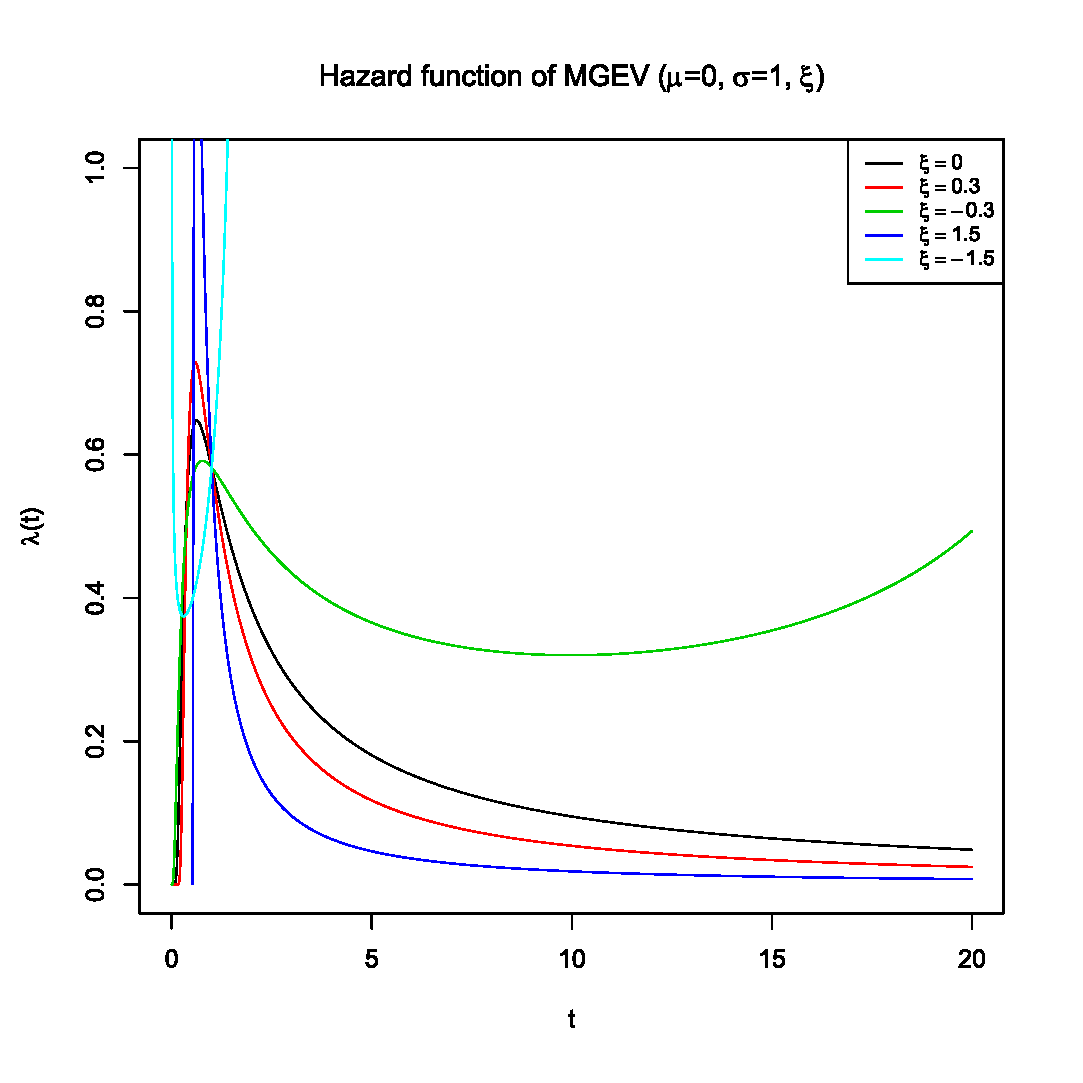
\includegraphics[width=7cm]{fig1.eps}
}
\subfloat[]{
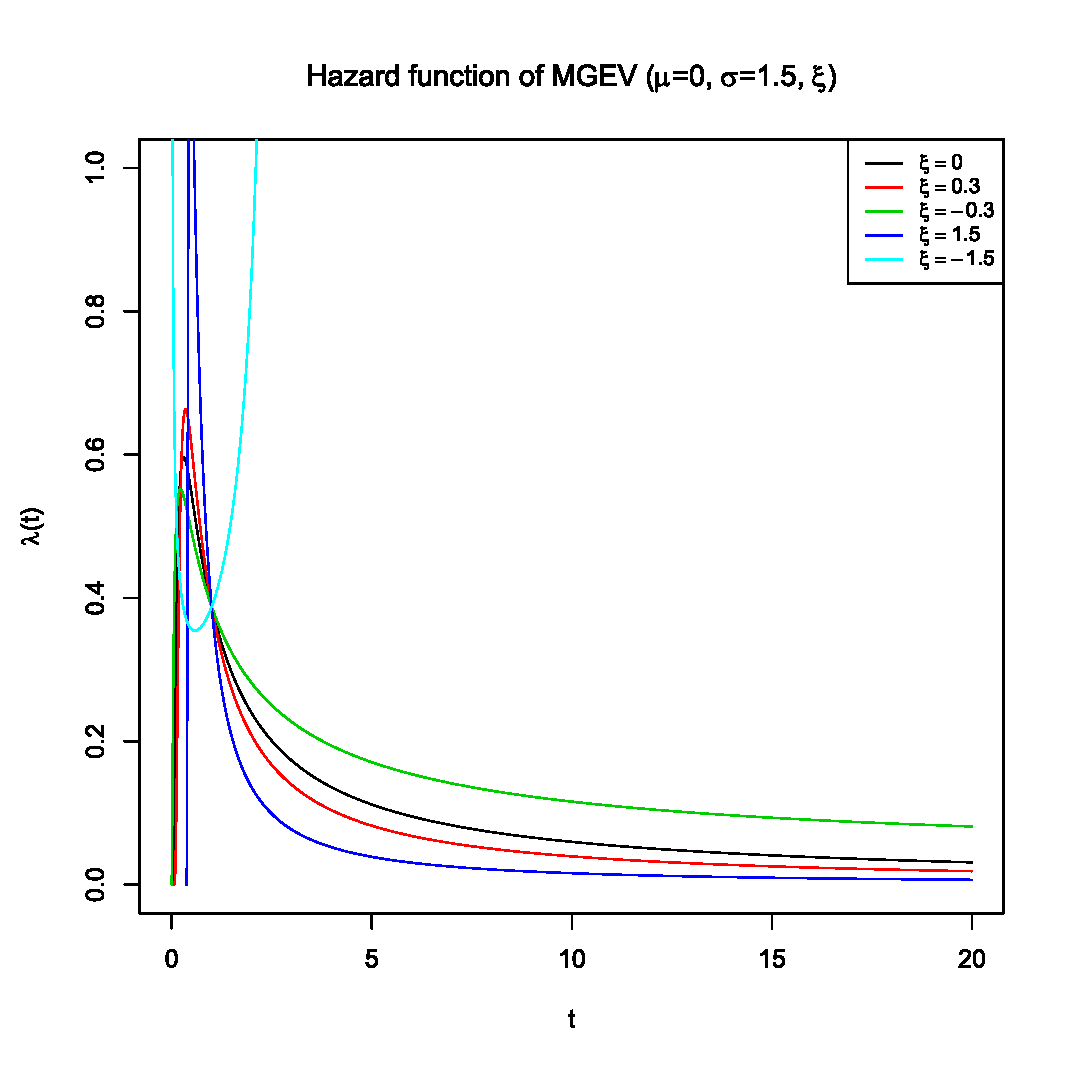
\includegraphics[width=7cm]{fig2.eps}
}
\hspace{0mm}
\subfloat[]{
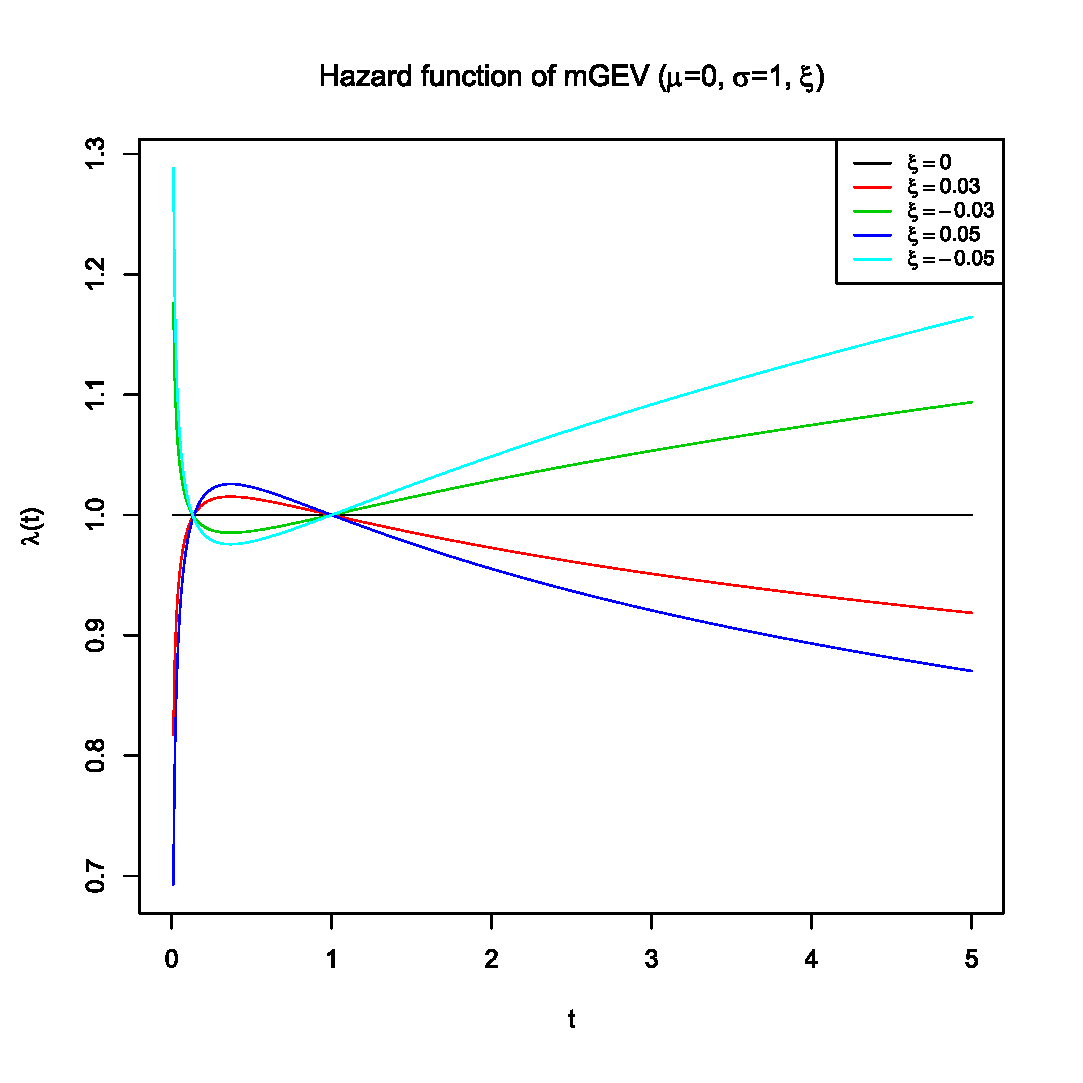
\includegraphics[width=7cm]{fig3.eps}
}
\subfloat[]{
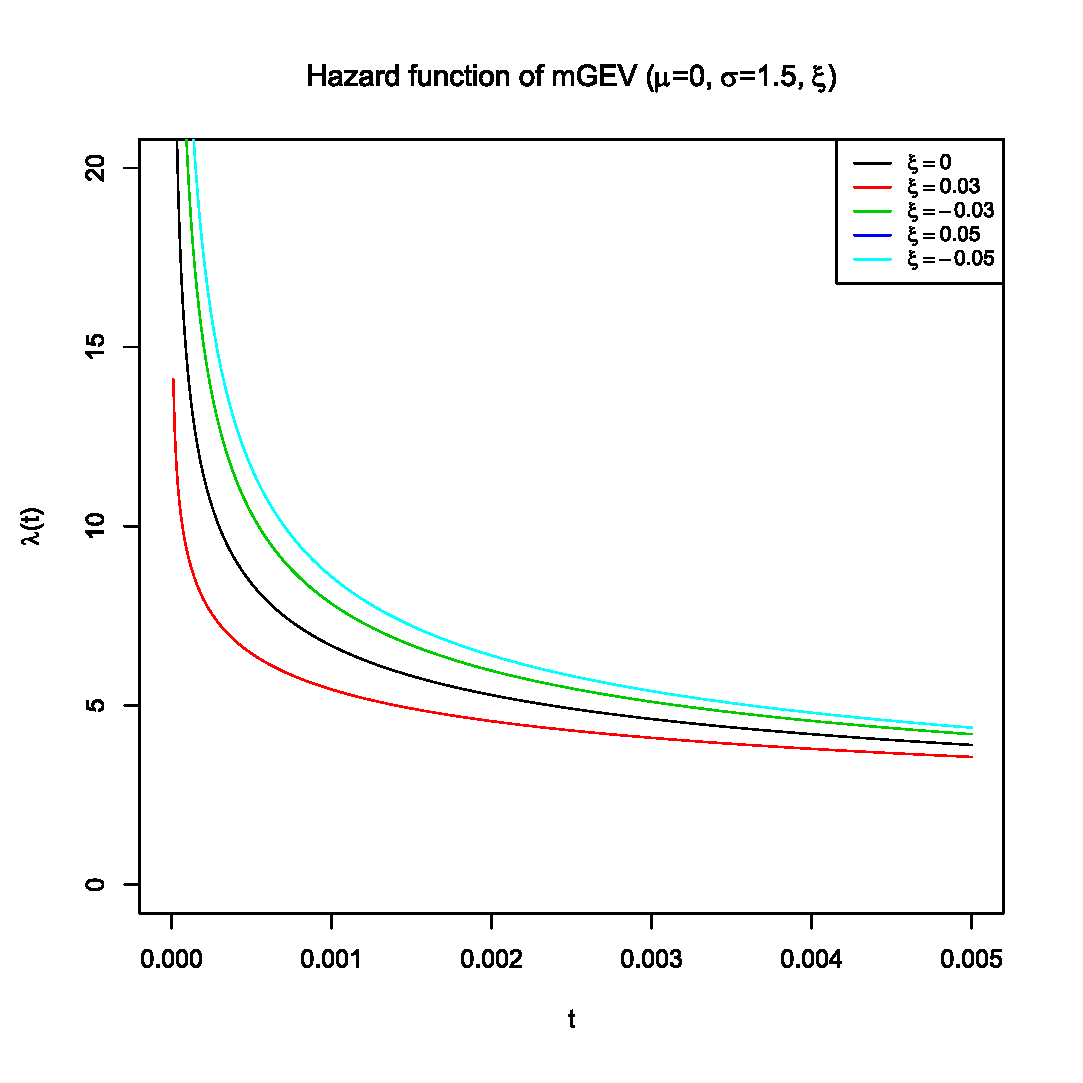
\includegraphics[width=7cm]{fig4.eps}
}
\caption{\\1(a) Hazard functions of the generalized extreme value distribution for $\mbox{MGEV}(\mu=0,\sigma=1,\xi)$ for different values of $\xi$.\\ 1(b) Hazard functions of the generalized extreme value distribution for $\mbox{MGEV}(\mu=0,\sigma=1.5,\xi)$ for different values of $\xi$.\\1(c) Hazard functions of the generalized extreme value distribution for $\mbox{mGEV}(\mu=0,\sigma=1,\xi)$ for different values of $\xi$.\\ 1(d) Hazard functions of the generalized extreme value distribution for $\mbox{mGEV}(\mu=0,\sigma=1.5,\xi)$ for different values of$\xi$ .}
\label{fig:test}
\end{figure*}


\begin{figure*}[!p]
\centering
\subfloat[]{
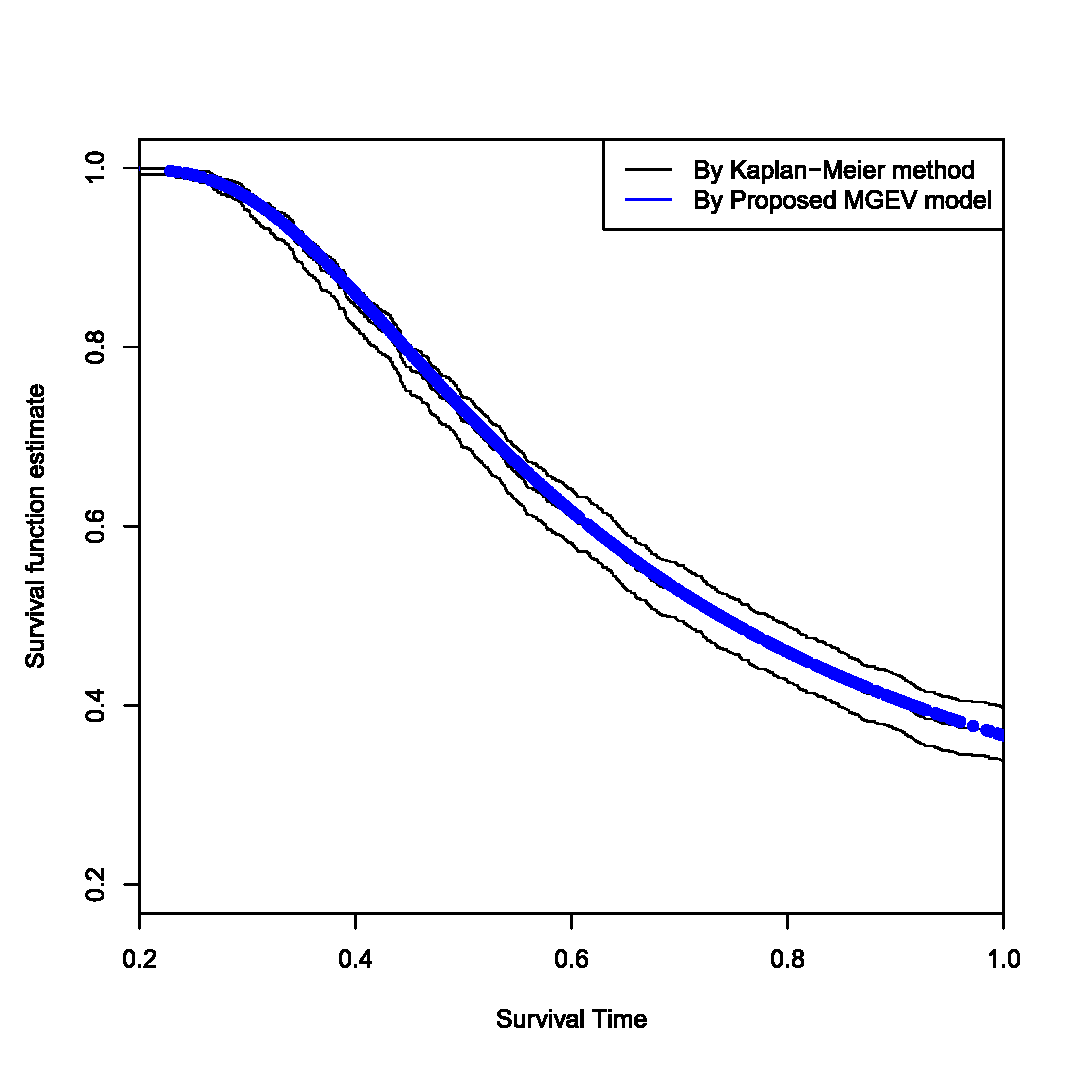
\includegraphics[width=7cm]{fig5.eps}
}
\subfloat[]{
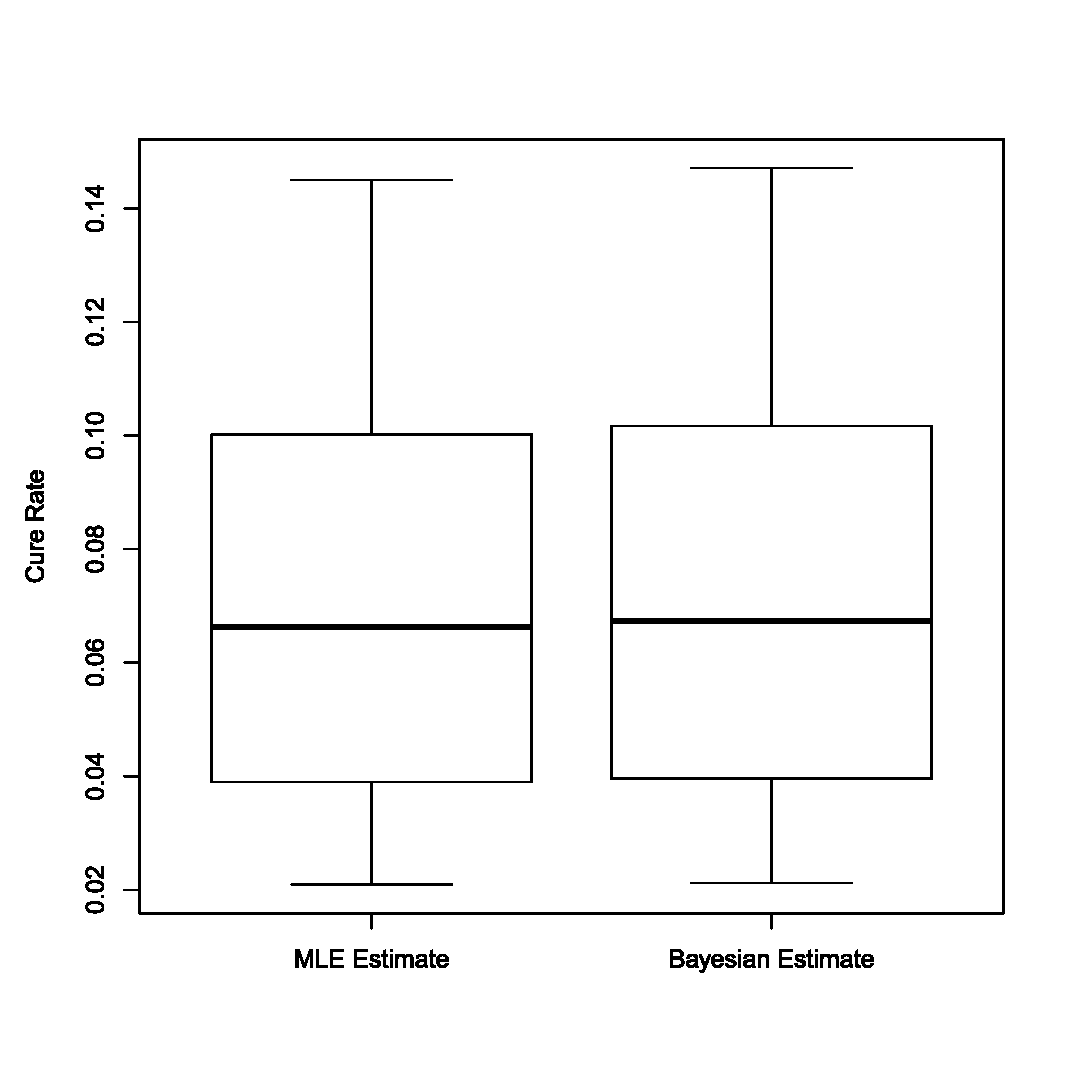
\includegraphics[width=7cm]{fig6.eps}
}
\hspace{0mm}
\subfloat[]{
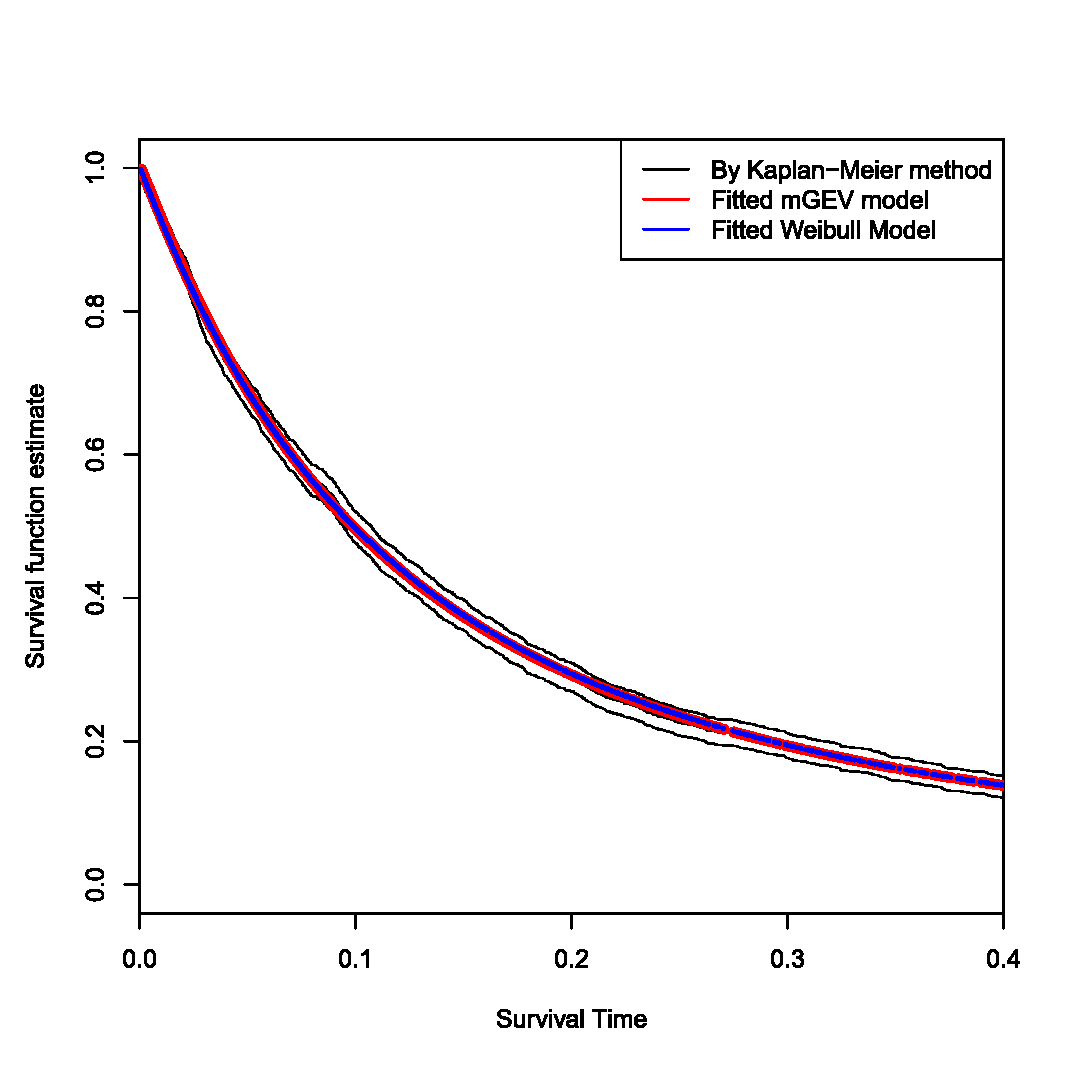
\includegraphics[width=7cm]{fig7.eps}
}
\subfloat[]{
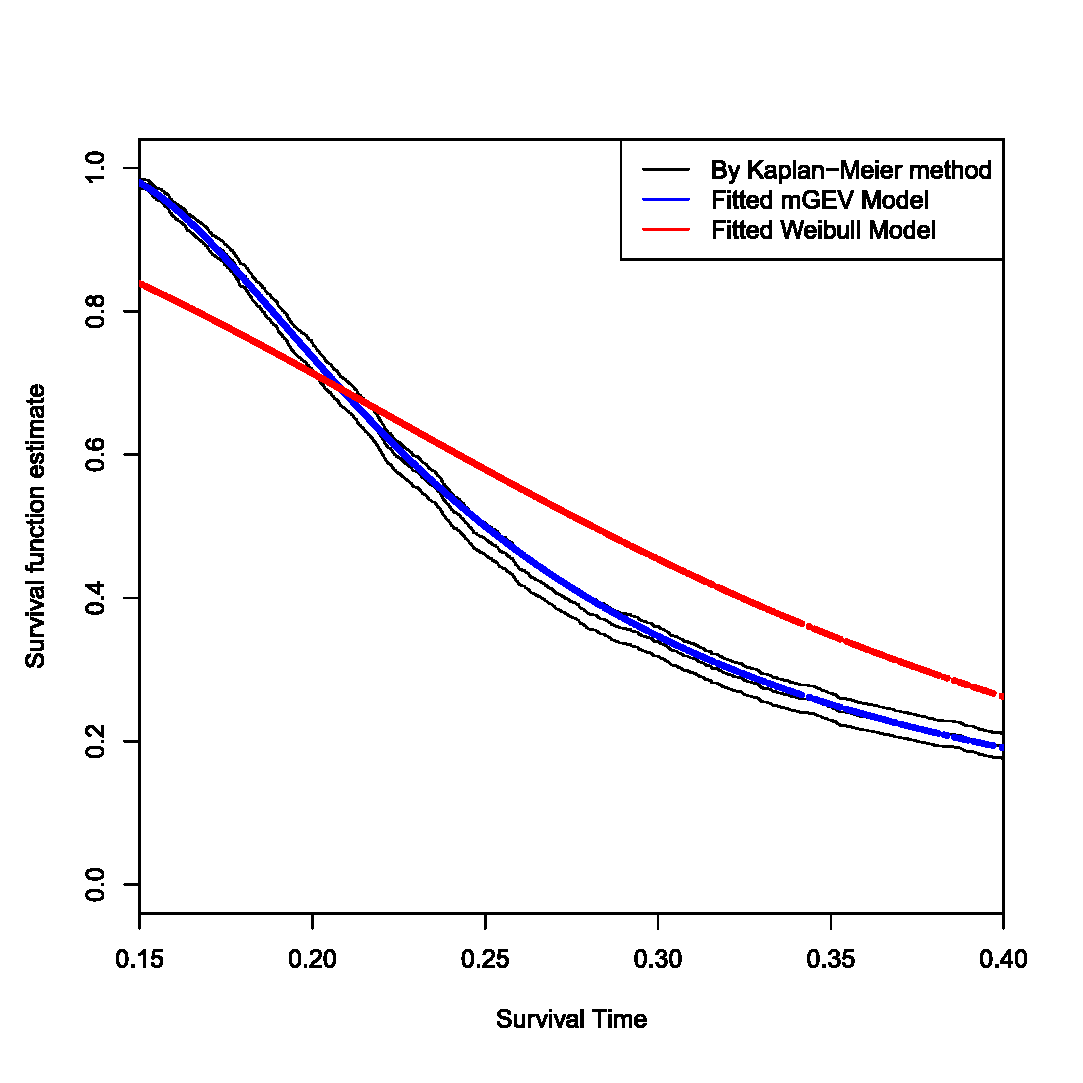
\includegraphics[width=7cm]{fig8.eps}
}
\caption{\\2(a) Estimated survival curves for the simulated data by Kaplan-Meier method (solid
line is the estimate, dashed lines are 95\% confidence band for the
survival function) and the proposed model(the blue line).\\ 2(b) Box plots of the cure rates for the simulated data.\\ 2(c) Estimated survival Curves for the simulated model $\mbox{Weibull(\ensuremath{\alpha}=1.03,\ensuremath{\lambda}=1)}$ by Kaplan-Meier method (solid line is the estimate, dashed lines are 95\% confidence band for the survival function) and the fitting models $\mbox{mGEV}(\mu=0,\sigma=1,\xi)$ (the red line) and the $\mbox{Weibull(\ensuremath{\alpha},\ensuremath{\lambda}=1)}$ (the blue line).\\ 2(d) Estimated survival Curves for the simulated model $\mbox{mGEV}(\mu=0,\sigma=1,\xi=0.5)$ by Kaplan-Meier method (solid line is the estimate, dashed lines are 95\% confidence band for the survival function) and the proposed model $\mbox{Weibull(\ensuremath{\alpha},\ensuremath{\lambda}=1)}$ (the red line) and the $\mbox{mGEV}(\mu=0,\sigma=1,\xi)$(the blue line).}
\label{fig:test}
\end{figure*}

\begin{figure*}[!p]
\centering
\subfloat[]{
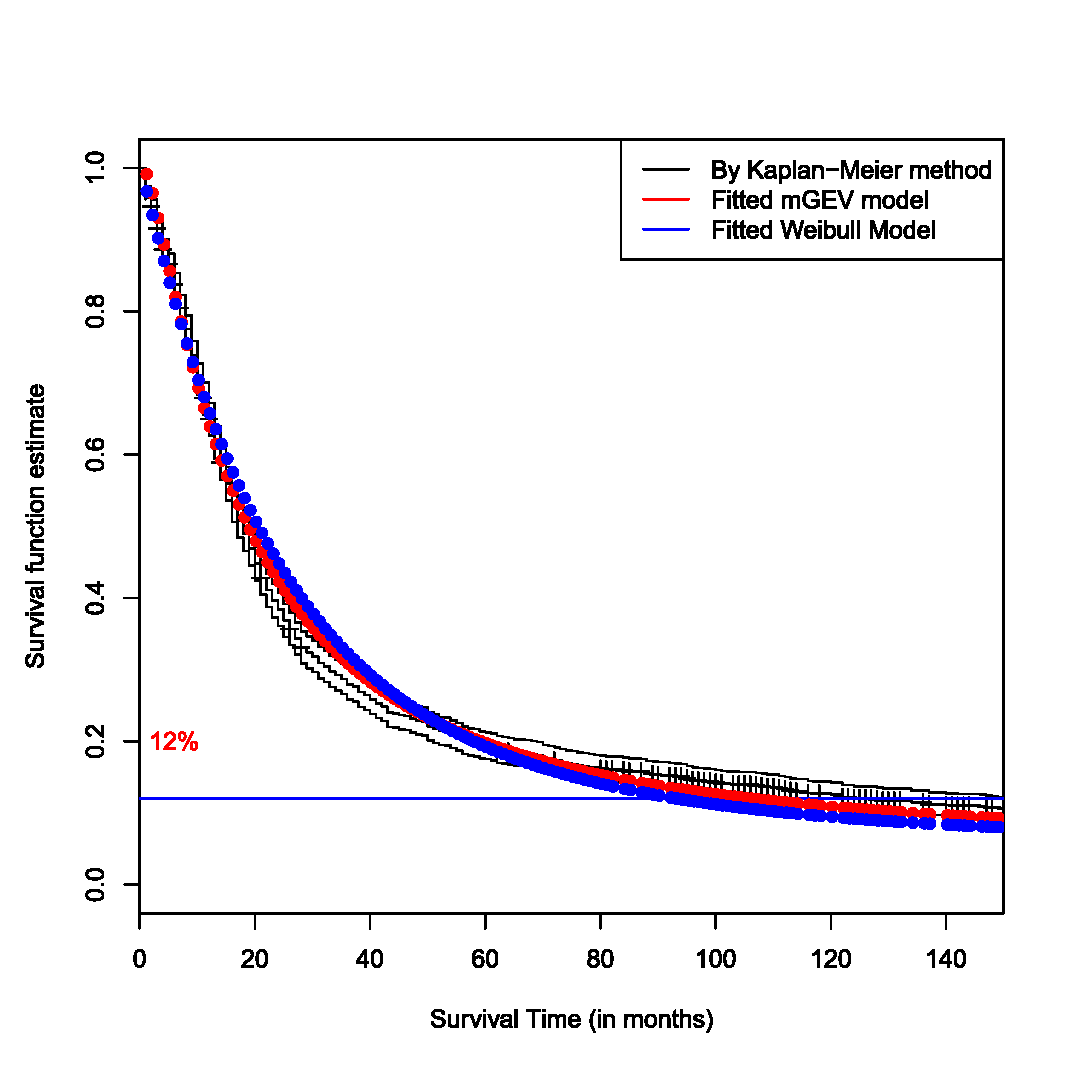
\includegraphics[width=7cm]{fig9.eps}
}
\subfloat[]{
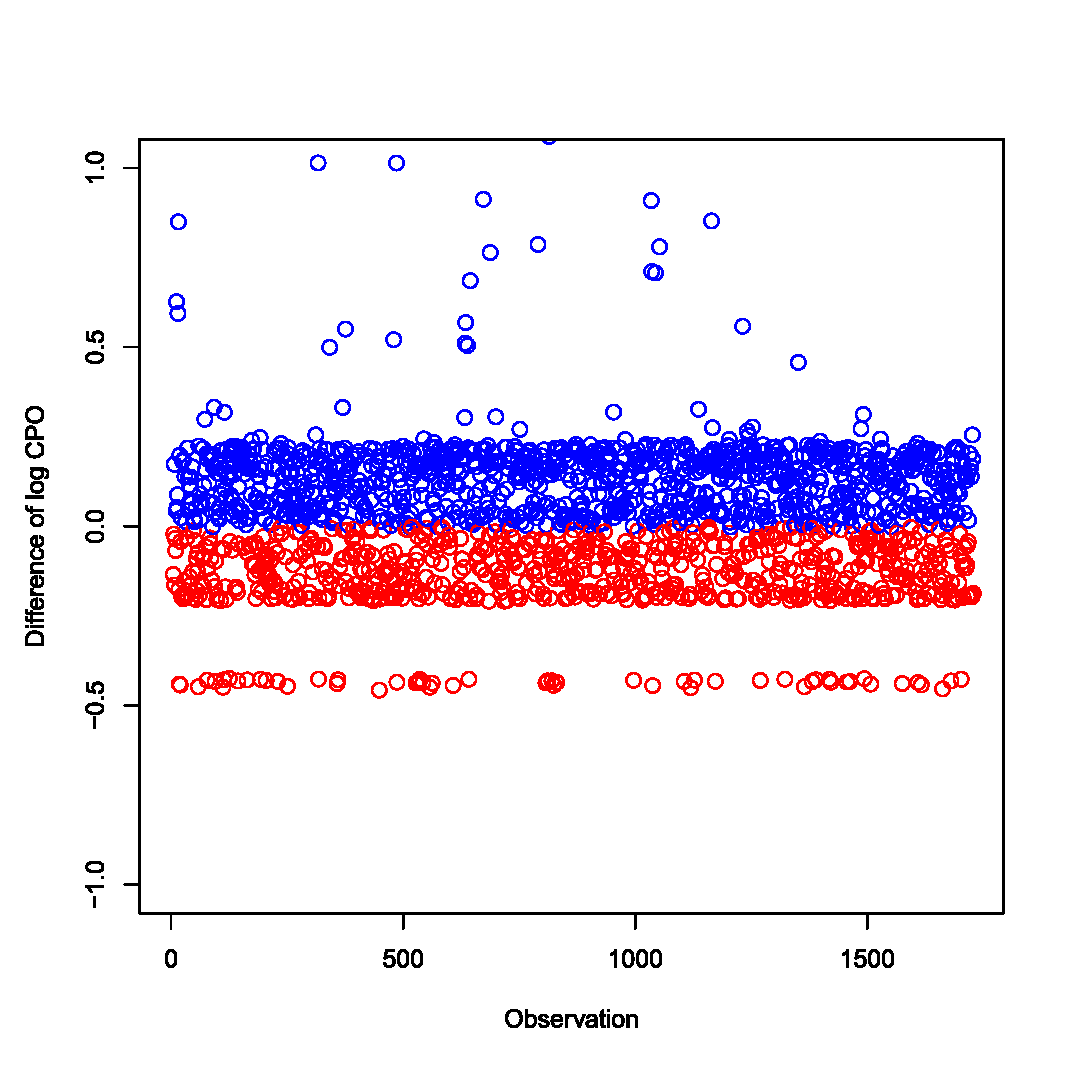
\includegraphics[width=7cm]{fig10.eps}
}
\caption{\\3(a) Estimated survival curves for the GBM data by Kaplan-Meier method(solid
line is the estimate, dashed lines are 95\% confidence band for the
survival function), the fitted Weibull Model(the blue line) and the proposed mGEV model(the red line).\\ 3(b) Plot of difference of the log CPO between mGEV and Weibull Model for the GBM cancer data.}
\label{fig:test}
\end{figure*}

%% For one-column wide figures use
%\begin{figure}
%% Use the relevant command to insert your figure file.
%% For example, with the graphicx package use
%  \includegraphics{example.eps}
%% figure caption is below the figure
%\caption{Please write your figure caption here}
%\label{fig:1}       % Give a unique label
%\end{figure}
%%
%% For two-column wide figures use
%\begin{figure*}
%% Use the relevant command to insert your figure file.
%% For example, with the graphicx package use
%  \includegraphics[width=0.75\textwidth]{example.eps}
%% figure caption is below the figure
%\caption{Please write your figure caption here}
%\label{fig:2}       % Give a unique label
%\end{figure*}
%
\newpage

\begin{table}[!p]
\caption{MLE's \& Bayesian Estimates of the model parameters: $\beta_{0},\ \beta_{1},\ \xi.$}
\centering{}%
\begin{tabular}{ccccc}
\hline
Parameter  & MLE  & SD  & Posterior Mean & 95\% HPD interval\tabularnewline
\hline
Intercept  & 1.003  & 0.037  & 0.998 & (0.918, 1.056)\tabularnewline
Age  & 0.201  & 0.036  & 0.203   & (0.132, 0.276)\tabularnewline
$\xi$  & 0.291  & 0.024 & 0.289  & (0.234, 0.343)\tabularnewline
\hline
\end{tabular}
\end{table}

\begin{table}[!p]
{\small \caption{Comparison of Posterior Inference between Weibull distribution and mGEV distribution.}
}{\small \par}
\centering{}{\small }%
\begin{tabular}{ccccc}
\hline
\hline
{\small Simulated Model } & {\small Fitting Model } & {\small Parameter } & {\small Posterior Mean } & {\small HPD interval}\tabularnewline
\hline
 &  & {\small $\beta_{0}$ } & {\small 1.989 } & {\small (1.936, 2.039)}\tabularnewline
 {\small $\mbox{Weibull}(\alpha=1.03,\lambda=1)$ } & {{\small $\mbox{mGEV}(\mu=0,\sigma=1,\xi)$ }} & {\small
 $\beta_{1}$ } & {\small 0.628 }  & {\small (0.581, 0.679)}\tabularnewline
 &  & {\small $\xi$ } & {\small 0.011 } & {\small (-0.002, 0.023)}\tabularnewline

 &  & {\small $\beta_{0}$ } & {\small 1.999 } & {\small (1.845, 2.153)}\tabularnewline
 {{\small $\mbox{Weibull}(\alpha=1.03,\lambda=1)$ }} & {{\small $\mbox{Weibull}(\alpha,\lambda=1)$ }} & {\small
 $\beta_{1}$ } & {\small 0.645 }  & {\small (0.542, 0.758)}\tabularnewline
 & & {\small $\alpha$ } & {\small 1.021 } & {\small (0.951, 1.101)}\tabularnewline



 &  & {\small $\beta_{0}$ } & {\small 3.086 }  & {\small (2.835, 3.306)}\tabularnewline
 {{\small $\mbox{mGEV}(\mu=0,\sigma=1,\xi=0.5)$ }} & {{\small $\mbox{Weibull}(\alpha,\lambda=1)$ }} & {\small
 $\beta_{1}$ } & {\small 0.665 } & {\small (0.544, 0.786)}\tabularnewline
 &  & {\small $\alpha$ } & {\small 2.735 } & {\small (2.486, 2.934)}\tabularnewline

 &  & {\small $\beta_{0}$ } & {\small 1.998 }  & {\small (1.945, 2.044)}\tabularnewline
 {{\small $\mbox{mGEV}(\mu=0,\sigma=1,\xi=0.5)$ }} & {{\small $\mbox{mGEV}(\mu=0,\sigma=1,\xi)$ }} & {\small $\beta_{1}$ } & {\small 0.588 } & {\small
 (0.540,0.633)}\tabularnewline
 &  & {\small $\xi$ } & {\small 0.499 } & {\small (0.496, 0.501)}\tabularnewline
\hline
\end{tabular}
\end{table}

\renewcommand{\arraystretch}{.5}
\setlength{\tabcolsep}{10pt}
\begin{table}[!p]
%\captionsetup{justification=centering}
{\small \caption{Model Fitting Comparison of mGEV, MGEV, Weibull and Exponentiated Weibull distributions.}}{\small \par}
\centering{}{\small }%
\begin{tabular}{ccccc}
\hline
\hline\\
&&&{Fitted}&\\
\cline{3-5}\\
{Generated}& & {\small mGEV}& {\small MGEV}& {\small Weibull}\\ \hline\\
& {\small $LPML$}&{\small 1742.649}&{\small 1562.961}& {\small 1301.597}\tabularnewline
{\small $\mbox {mGEV}$}&&&&\tabularnewline
& {\small $DIC$}&{\small -3485.159} &{\small -3126.306}&{\small -2603.715}\\\\
& {\small $LPML$}&{\small 174.949}&{\small	695.359}	&{\small -392.934}\tabularnewline
{\small $\mbox{MGEV}$}&&&&\tabularnewline
& {\small $DIC$} &{\small -348.746}	&{\small -1390.719} &{\small	798.289}\\\\
& {\small $LPML$}&{\small 1611.027}&{\small	1590.493}	&{\small 1595.899}\tabularnewline
{\small $\mbox{Weibull}$}&&&& \tabularnewline
& {\small $DIC$} &{\small -3222.066} &{\small -3181.773} &{\small -3192.217}\\\\
& {\small $LPML$}&{\small 424.115}&{\small	476.069}	&{\small 482.26}\tabularnewline
{\small $\mbox{Exponentiated Weibull}$}&&&& \tabularnewline
& {\small $DIC$} &{\small -850.013} &{\small -952.832} &{\small -964.704}\\
\hline
\end{tabular}
\end{table}

\renewcommand{\arraystretch}{1}
\setlength{\tabcolsep}{6pt}
\begin{table}[!p]
\caption{Influence Diagnostics for the mGEV model.}
\centering{}%
\begin{tabular}{ccccccc}
\hline
Data set & Perturbed Cases & $\beta_0$ & $\beta_1$ & $\xi$ & DIC & LPML \tabularnewline
\hline
a & none & 2.002 & 0.595 & 0.501 & -3494.89 & 1747.411\tabularnewline
b & 1 & 1.996 & 0.587 & 0.501   & -3473.727 & 1736.797\tabularnewline
c & 200 & 1.995 & 0.585 & 0.501 & -3477.262 & 1738.623\tabularnewline
d & 600 & 1.998 & 0.592 & 0.501 & -3479.290 & 1739.632\tabularnewline
e & ${1,200}$ & 1.994 & 0.592 & 0.501 & -3461.795 & 1730.878\tabularnewline
f & ${1,200,600}$ & 1.991 & 0.574 & 0.501 & -3441.219 & 1720.494\tabularnewline
\hline
\end{tabular}
\end{table}

\begin{table}[!p]
\caption{Influence Diagnostics for the Weibull model.}
\centering{}%
\begin{tabular}{ccccccc}
\hline
Data set & Perturbed Cases & $\beta_0$ & $\beta_1$ & $\alpha$ & DIC & LPML \tabularnewline
\hline
\hline
a & none & 1.989 & 0.599 & 1.019 & -3233.66 & 1616.325\tabularnewline
b & 1 & 1.986 & 0.597 & 1.021   & -3209.603 & 1604.433\tabularnewline
c & 200 & 1.986 & 0.597 & 1.019 & -3212.707 & 1605.953\tabularnewline
d & 600 & 1.983 & 0.594 & 1.019 & -3207.631 & 1603.393\tabularnewline
e & ${1,200}$ & 1.985 & 0.597 & 1.021 & -3205.160 & 1602.221\tabularnewline
f & ${1,200,600}$ & 1.979 & 0.598 & 1.017 & -3197.366 & 1598.312\tabularnewline
\hline
\end{tabular}
\end{table}

\begin{table}[!p]
{\small \caption{Summary of the GBM Cancer Data.}
}{\small \par}

{\small \centering{}}%
\begin{tabular}{cccccc}
\hline
\hline
{\small Survival time(y) (months) } & {\small Status(freq) } & {\small Age (years) } & {\small
Gender (freq) } & {\small Radiation (freq) } & {\small Marital status(freq)}\tabularnewline
\hline
{\small Median 18 } & {\small Censored 182 } & {\small Mean 31.4 } & {\small Male 1053 } & {\small
Had 1453 } & {\small Married 876}\tabularnewline
{\small IQR 32 } & {\small Death 1543 } & {\small 10 } & {\small Female 672 } & {\small
None 333 } & {\small Other 897}\tabularnewline
\hline
\end{tabular}
\end{table}

\begin{table}[!p]
\caption{GBM Data: Posterior Estimates of the mGEV Model Parameters with covariates.}
\centering{}%
\begin{tabular}{cccc}
\hline
\hline
Variable & Posterior mean & Posterior SD & $95\%$ HPD interval\tabularnewline
\hline
$\mu$ & 4.315 & 0.087 & (4.145, 4.485)\tabularnewline
$\sigma$ & 1.203 & 0.052 & (1.102, 1.309)\tabularnewline
$\xi$ & 0.186 & 0.017 & (0.153, 0.216)\tabularnewline
Age & 0.033 & 0.002 & (0.028, 0.037)\tabularnewline
Had Radiation & -0.096 & 0.062 & (-0.218, 0.018)\tabularnewline
Marital Status & -0.079 & 0.056 & (-0.188, 0.034)\tabularnewline
Gender & 0.221 & 0.050 & (0.127, 0.325)\tabularnewline
\hline
\end{tabular}
\end{table}

\begin{table}[!p]
\caption{GBM Data: Posterior Estimates of the Weibull Model Parameters with covariates.}
\centering{}%
\begin{tabular}{cccc}
\hline
\hline
Variable & Posterior mean & Posterior SD & $95\%$ HPD interval\tabularnewline
\hline
$\lambda$ & 66.216 & 0.449 & (65.368, 66.870)\tabularnewline
$\alpha$ & 1.104 & 0.020 & ( 1.065, 1.143)\tabularnewline
Age & 0.031 & 0.003 & (0.025, 0.035)\tabularnewline
Had Radiation & -0.067 & 0.074 & (-0.193, 0.098)\tabularnewline
Marital Status & -0.076 & 0.055 & (-0.173, 0.042)\tabularnewline
Gender & 0.225 & 0.057 & (0.113, 0.335)\tabularnewline
\hline
\end{tabular}
\end{table}

\begin{table}[!p]
{\small \caption{Model Comparison between Fitted mGEV distribution and Fitted Weibull distribution.}
}{\small \par}
\centering{}{\small }%
\begin{tabular}{ccccc}
\hline
{\small Fitted Model }& {DIC } & {LPML } \tabularnewline
\hline
{$\mbox{mGEV}(\mu,\sigma,\xi)$ } & { 14177.23 } & { -7088.581 } \tabularnewline
{$\mbox{Weibull}(\alpha,\lambda)$ }  & {14299.21 } & {-7150.145 } \tabularnewline
\hline
\end{tabular}
\end{table}

\end{document}
% end of file template.tex